%\VignetteDepends{knitr}
%\VignetteIndexEntry{An introduction to GAGA}
%\VignetteCompiler{knitr}
%\VignetteEngine{knitr::knitr}

\documentclass{article}

% LaTeX packages 
\usepackage{hyperref} % For hyperlinks\
\usepackage{float} % for floating images
\usepackage{alltt} % for verbatim blocks of text
\usepackage{xcolor} % to define custom colours

\definecolor{icrgreen}{HTML}{C9DD03}
\definecolor{icryellow}{HTML}{FFD602}
\definecolor{icrorange}{HTML}{F9A100}
\definecolor{icrpink}{HTML}{EE7EA6}
\definecolor{icrred}{HTML}{A71930}

% This block sets all links to be black and removes the hideous coloured boxes around them
\hypersetup{
    colorlinks=true,
    linkcolor=black,
    citecolor=black,
    filecolor=black,
    urlcolor=black,
}

\usepackage{Sweave}
\begin{document}
\Sconcordance{concordance:GAGA_vignette.tex:GAGA_vignette.Rnw:%
1 11 1 1 0 14 1 1 3 2 0 1 1 1 2 4 0 1 2 20 1 1 3 2 0 1 3 1 0 1 4 12 0 1 %
2 1 3 5 0 1 2 3 1 13 0 1 12 12 1}


\title{An introduction to GAGA}
%\author{Alex Murison and Christopher P Wardell \\ Alexander.Murison@icr.ac.uk, Christopher.Wardell@icr.ac.uk} % as single line
\author{
  Alex Murison\\
  Alexander.Murison@icr.ac.uk
  \and
  Christopher P Wardell\\
  Christopher.Wardell@icr.ac.uk
}
\maketitle

This vignette serves as an introduction to the R package GAGA.  It covers the basic use cases and usage of the package, explaining the input and output and contains several worked examples.  If you use this package, please cite: (CITATION).

\paragraph{Installation:} The latest stable version can be installed from Bioconductor here...
 
\begin{Schunk}
\begin{Sinput}
> ## Install
> source("http://bioconductor.org/biocLite.R")
> biocLite("GAGA")
> ## Load
> library(GAGA)
\end{Sinput}
\end{Schunk}

The latest development version can be cloned from our GitHub:\\ \texttt{\href{https://github.com/MurisonWardell}{https://github.com/MurisonWardell}} but must be built from source.

\pagebreak
\tableofcontents
\pagebreak

\section{Overview}
\subsection{Introduction}
We work extensively with sequencing data, particularly next-generation sequencing data from tumour-normal pairs.  The tumour genome contains many single nucleotide variants (SNVs) which are single-base differences between the tumour sample and the reference genome.  These can be separated into two groups:

\begin{enumerate}
   \item SNVs shared between tumour and normal samples.  These are germline variants and were present before the tumour
   \item SNVs only present in the tumour sample.  These are somatic mutations
\end{enumerate}

Tumours are known to be heterogeneous populations of related cells and in any given tumour sample there may be differing proportions of cells that contain certain SNVs.  These proportions can be calculated for each SNV in turn using the number of supporting reads, the read depth and the copy number of that region.  These proportions are termed the cancer cell fraction (CCF) and range between 0 (no cells contain the SNV in that sample) to 1 (all cells contain the SNV in that sample).

The SNV CCF values can be explained as a mixture of a number of related clones.  We know that SNVs are heritable characteristics between clones and that new clones arise and go extinct over time.

As these mixtures are the product of evolutionary processes it seemed appropriate to use genetic algorithms to infer their ancestry and composition.

\subsection{Genetic algorithms}
Genetic algorithms (GAs) are stochastic heuristic optimisation algorithms.  A population of potential solutions is generated and using a scoring function is compared to the observed data.  Solutions that best explain the observed data are allowed to reproduce with one another.  Reproduction allows both the recombination of solutions from different individuals and also the possibility of mutations.

GAs are particularly useful when a brute-force approach is undesirable or impractical, for example when the search space is very large.  An important consideration is that the search space may contain multiple solutions that exist as local minima and these may be difficult to escape, even with a high mutation rate.  \textbf{It is therefore imperative to run GAGA multiple times and select the best-scoring solution}.  Further details are discussed in the Advanced GAGA usage and best practices section of the worked examples.

\subsection{GAGA input}
The main GAGA function (\emph{gaga()}) requires a data frame of observations as input.  Each row represents an SNV and each column represents a discrete sample separated by time or space. Every value must be a value between 0 and 1 and represents the proportion of individuals that contain that SNV.

\subsection{How GAGA encodes individuals and solutions}
Every individual in the population is encoded as a character string.  Consider the following solution to an included data set.  It contains three clones and three SNVs.  The solution encodes a phylogeny, the proportion of each clone in each sample and the clone in which each SNV first occurred.  Let there be {\color{icrpink}s} samples and {\color{icrred}k} clones.
\newline
\newline
{\raggedright{}\texttt{{\color{icrgreen}0  1  2 }{\color{icryellow} 5  0  0  3  7  0   0   1   4 }{\color{icrorange} 1   2   3 }}}
\newline
\newline
\texttt{{\color{icrgreen}0  1  2 }}: The first {\color{icrred}k} characters encode the position in the phylogeny of each clone.  In this example, the first element is the root (hence 0), the second is descended from the first and third is descended from the second.  If the second and third clones were both descended from the first clone, the phylogeny would be \texttt{0 1 1}.
\newline
\newline
\texttt{{\color{icryellow}5  0  0  3  7  0   0   1   4 }}: The next {\color{icrred}k}*{\color{icrpink}s} characters encode the proportions.  Each block of {\color{icrred}k} characters encodes the proportions of each clone for the {\color{icrpink}s}th sample.  Proportions are generated by dividing the numbers in the block by their sum.  This example is explained below:

\begin{Schunk}
\begin{Sinput}
> ## First sample is reprented by first block of three digits
> ## First sample is 100% clone 1, 0% clone 2, 0% clone 3
> c(5,0,0)/sum(c(5,0,0))
\end{Sinput}
\begin{Soutput}
[1] 1 0 0
\end{Soutput}
\begin{Sinput}
> ## Second sample is reprented by second block of three digits
> ## Second sample is 30% clone 1, 70% clone 2, 0% clone 3
> c(3,7,0)/sum(c(3,7,0))
\end{Sinput}
\begin{Soutput}
[1] 0.3 0.7 0.0
\end{Soutput}
\begin{Sinput}
> ## Third sample is reprented by third block of three digits
> ## Third sample is 0% clone 1, 20% clone 2, 80% clone 3
> c(0,1,4)/sum(c(0,1,4))
\end{Sinput}
\begin{Soutput}
[1] 0.0 0.2 0.8
\end{Soutput}
\end{Schunk}

\newline
\newline
{\raggedright{}\texttt{{\color{icrorange}1   2   3 }}: The final {\color{icrred}k} characters encodes the mutation matrix and the order of SNVs. In this example the first SNV occurred in clone 1 (and is inherited by its descendants), the second SNV occurred in clone 2 (and is inherited by its descendent) and SNV 3 occurred in clone 3.  If all SNVs occurred in clone 1, this string would be \texttt{1 1 1}.}

\subsection{GAGA mutation function}
The mutation function has been heavily modified in \texttt{GAGA} relative to the original in \texttt{GA}.  If an individual in the
population undergoes mutation there is an equal chance of it occurring in the phylogeny, proportion of clones or mutation matrix 
sections of the solution.

A mutation in the phylogeny section results in a new phylogeny being randomly assigned to the individual. A mutation in the proportion
section results in between 1 to {\color{icrred}k} increments or decrements to the assigned values.  This enhanced level of mutation
is required to help individuals escape from local minima.  A mutation in the mutation matrix section results in a single value being randomly assigned to a new clone.

Also, note that crosses between parents are not permitted in the phylogeny section of the solution.

\subsection{GAGA output}
The \texttt{gaga()} function returns an object of class \texttt{ga}.  Although this object can be interrogated manually, the easiest way to look at the results is to use the gagaReport() function.  The default output will produce the following files in the current working directory (where {\color{icrred}k}=number of clones, {\color{icrred}i}=number of solution and {\color{icrred}n}=total number of top-scoring solutions):

\begin{enumerate}
   \item png image: {\color{icrred}k}clones.solution{\color{icrred}i}of{\color{icrred}n}.phylogeny.png: the inferred phylogeny of the solution 
   \item png image: {\color{icrred}k}clones.solution{\color{icrred}i}of{\color{icrred}n}.heatmap.png: a heatmap of the solution
   \item png image: {\color{icrred}k}clones.solution{\color{icrred}i}of{\color{icrred}n}.proportions.png: a stacked barplot of the proportion of each clone that composes each sample
   \item png image: {\color{icrred}k}clones.fitnessconvergence.png: the fitness convergence plot.  This can be used to ensure that GAGA is reaching convergence and being run for an appropriate number of generations
   \item text file: {\color{icrred}k}clones.complete.solution{\color{icrred}i}of{\color{icrred}n}.txt: the solution encoded as a string
   \item text file: {\color{icrred}k}clones.phylogeny.solution.{\color{icrred}i}of{\color{icrred}n}.txt: the phylogeny of the solution
   encoded as a matrix.  Note that these matrices are not directly compatible with the \emph{graph} R package
   \item text file: {\color{icrred}k}clones.mutation.matrix.{\color{icrred}i}of{\color{icrred}n}.txt: a binary matrix showing the
   presence or absence of each SNV in each clone
   \item text file: {\color{icrred}k}clones.proportions.solution.{\color{icrred}i}of{\color{icrred}n}.txt: the proportion of each 
   clone that composes each sample
\end{enumerate}

Note that in the event of multiple solutions scoring equally well, files for up to the top five solutions will be produced.

\begin{Schunk}
\begin{Sinput}
> ## Write results to files
> gagaReport(gaga_input_dataframe,gaga_output_object)
\end{Sinput}
\end{Schunk}


\section{Worked examples}
A number of sample data sets are distributed with the GAGA package and are discussed in order of increasing complexity.
\subsection{Example 1 - simple synthetic data}
A very small and simple synthetic data set is included.  To demonstrate that your GAGA installation is working, you can execute the following commands.  
\begin{Schunk}
\begin{Sinput}
> ## Load library
> library(GAGA)
> ## Load simple data set
> data("gaga_simple_data")
> ## There  are three columns (time points T0, T1 and T2)
> ## and three rows (mutations M1, M2, M3)
> gaga_simple_data
\end{Sinput}
\begin{Soutput}
   T0  T1  T2
M1  1 1.0 1.0
M2  0 0.7 1.0
M3  0 0.0 0.8
\end{Soutput}
\end{Schunk}

As we know the true number and relationship between the clones, we specify these and run the algorithm.  It should converge at the minimum score of zero quite quickly and exit after 200 generations of coverging at the highest fitness value.

\begin{Schunk}
\begin{Sinput}
> ## Execute gaga() function on the simple data set
> simpleDataSolution=gaga(gaga_simple_data, number_of_clones=3, nroot=1,iterations=1000)
\end{Sinput}
\end{Schunk}

We can view the highest scoring solution(s) by accessing the appropriate slot in the returned object.  For example:

\begin{Schunk}
\begin{Sinput}
> ## Access solution slot in returned object to show highest scoring solution(s)
> simpleDataSolution@solution
\end{Sinput}
\end{Schunk}
% Note; this R code snippet isn't in a regular knitr code block on purpose to make it appear as if it has been run
\begin{alltt}
     x1 x2 x3 x4 x5 x6 x7 x8 x9 x10 x11 x12 x13 x14 x15
[1,]  0  1  2  5  0  0  3  7  0   0   1   4   1   2   3
[2,]  0  1  2  7  0  0  3  7  0   0   1   4   1   2   3
[3,]  0  1  2  1  0  0  3  7  0   0   1   4   1   2   3
[4,]  0  1  2  6  0  0  3  7  0   0   1   4   1   2   3
[5,]  0  1  2  3  0  0  3  7  0   0   1   4   1   2   3
[6,]  0  1  2 11  0  0  3  7  0   0   1   4   1   2   3
[7,]  0  1  2 12  0  0  3  7  0   0   1   4   1   2   3
\end{alltt}

Note that it's possible for multiple solutions to have equally good fitness scores which may encode different phylogenies, mutation distributions or proportions.  However, in this case all of the solutions are numerically identical and exist because of the degeneracy in the way that the clonal proportions are encoded.

We can now examine the best solution(s) using the gagaReport() function.  

\begin{Schunk}
\begin{Sinput}
> ## Produce plots for the phylogeny, heatmap and proportions in turn
> gagaReport(gaga_simple_data,simpleDataSolution,outType="phylogeny")
> gagaReport(gaga_simple_data,simpleDataSolution,outType="heatmap")
> gagaReport(gaga_simple_data,simpleDataSolution,outType="proportion")
> ## Create output files representing the solution(s) in the current working directory
> gagaReport(gaga_simple_data,simpleDataSolution,outType="complete")
> ## In case you want to know the current working directory, it can be reported using this function:
> getwd()
\end{Sinput}
\end{Schunk}

You should see images like those below.  The colours used for clones are consistent between the phylogeny, the sidebar of the heatmap and the proportion barplot.

\begin{figure}[H]
    \centering
    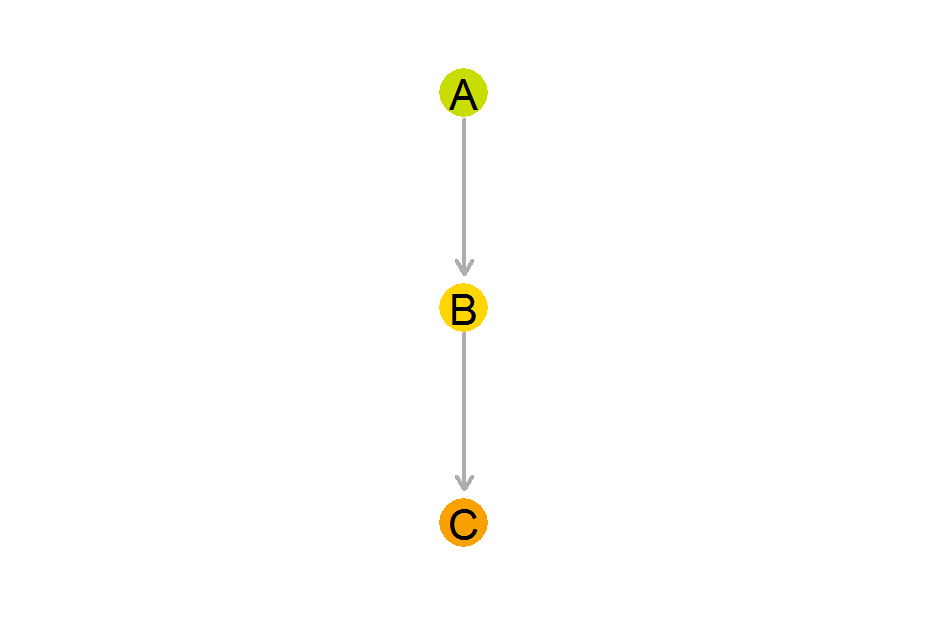
\includegraphics{gaga_simple_data_phylogeny.png}
    \caption{The phylogeny of the optimum solution to the simple data set.  There is a single root (clone A) which gives rise to clone B which gives rise to clone C.}
\end{figure}

\begin{figure}[H]
   \centering
       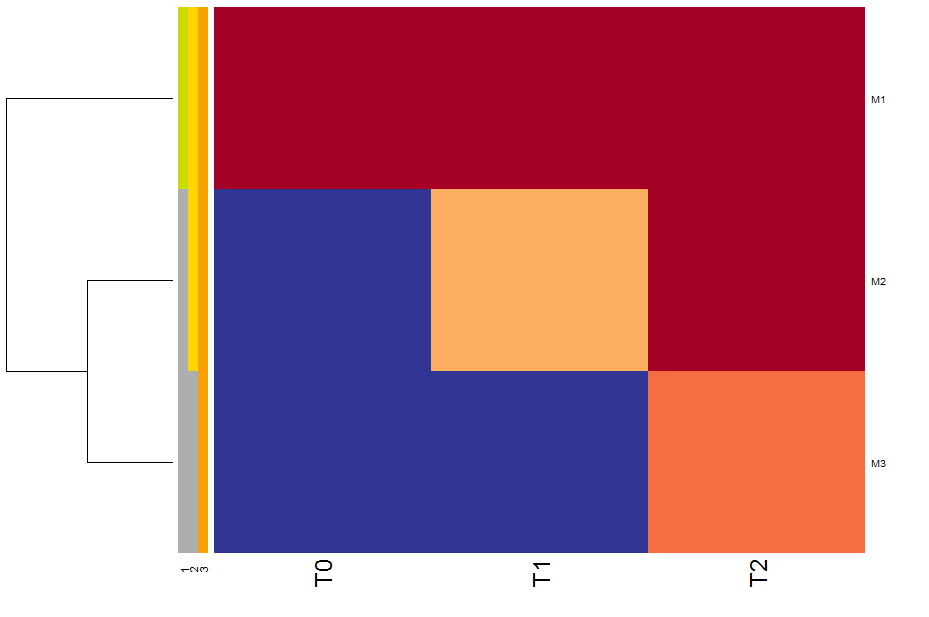
\includegraphics{gaga_simple_data_heatmap}
   \caption{The input data has been clustered using the heatmap.plus package.  The colour scale goes from blue (low values) through yellow to red (high values).
   The coloured sidebar shows which clones contain which mutations.  For example, M1 is contained by all clones, whereas M3 is contained only by clone C.}
\end{figure}

\begin{figure}[H]
   \centering
       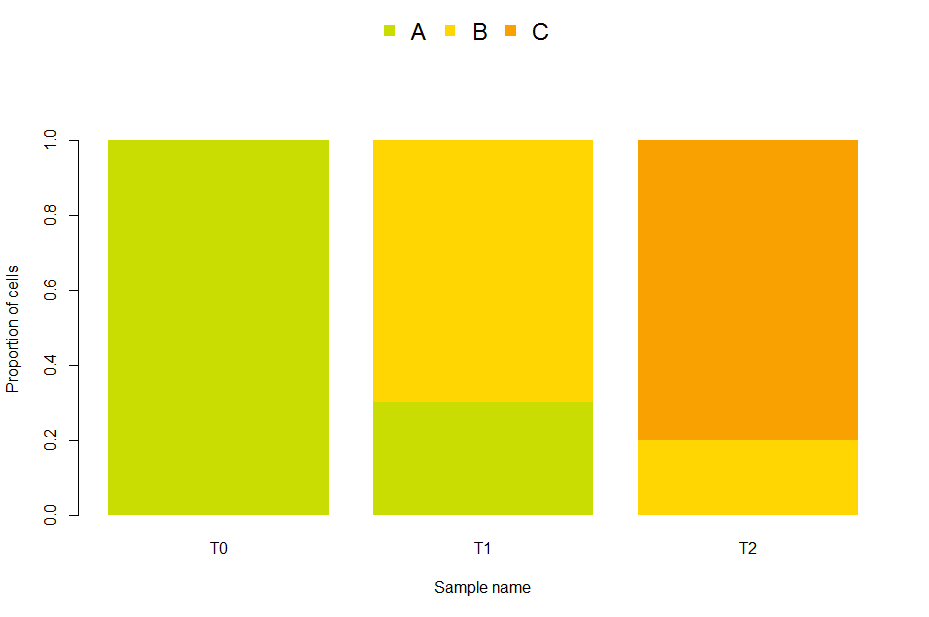
\includegraphics{gaga_simple_data_proportions}
   \caption{The proportions of each clone in each sample of the simple data set.  Sample T0 is composed entirely of clone A, whereas sample T1 is an unequal mixture of 
   clones A and B, while sample T2 is an unequal mixture of clones B and C.}
\end{figure}

\subsection{Example 2 - synthetic data containing a hidden clone}
The second synthetic data set demonstrates the ability of GAGA to infer intermediate clones that are not explicitly detected in the input data and therefore "hidden".

\begin{Schunk}
\begin{Sinput}
> ## Load library
> library(GAGA)
> ## Load hidden data set
> data("gaga_hidden_data")
> ## There  are three columns (time points T0, T1 and T2)
> ## and five rows (mutations M1, M2, M3, M4 and M5)
> gaga_hidden_data
\end{Sinput}
\begin{Soutput}
   T0  T1  T2
M1  1 1.0 1.0
M2  0 0.5 1.0
M3  0 0.3 0.7
M4  0 0.2 0.3
M5  0 0.0 0.6
\end{Soutput}
\end{Schunk}

\begin{Schunk}
\begin{Sinput}
> ## Execute gaga() function on the hidden data set
> hiddenDataSolution=gaga(gaga_hidden_data, number_of_clones=5, nroot=1,iterations=3000)
> ## Access solution slot in returned object to show highest scoring solution(s)
> ## This solution's score is -0.02500000
> hiddenDataSolution@solution
\end{Sinput}
\end{Schunk}
% Note; this R code snippet isn't in a regular knitr code block on purpose to make it appear as if it has been run
\begin{alltt}
     x1 x2 x3 x4 x5 x6 x7 x8 x9 x10 x11 x12 x13 x14 x15 x16 x17 x18 x19 x20 x21 x22 x23 x24 x25
[1,]  0  1  2  2  4 29  0  0  0   0   8   0   3   5   0   0   0   6   2  12   1   2   4   3   5
\end{alltt}

\begin{Schunk}
\begin{Sinput}
> ## Produce plots for the phylogeny, heatmap and proportions in turn
> gagaReport(gaga_hidden_data,hiddenDataSolution,outType="phylogeny")
> gagaReport(gaga_hidden_data,hiddenDataSolution,outType="heatmap")
> gagaReport(gaga_hidden_data,hiddenDataSolution,outType="proportion")
> ## Create output files representing the solution(s) in the current working directory
> gagaReport(gaga_simple_data,simpleDataSolution,outType="complete")
\end{Sinput}
\end{Schunk}

\begin{figure}[H]
    \centering
    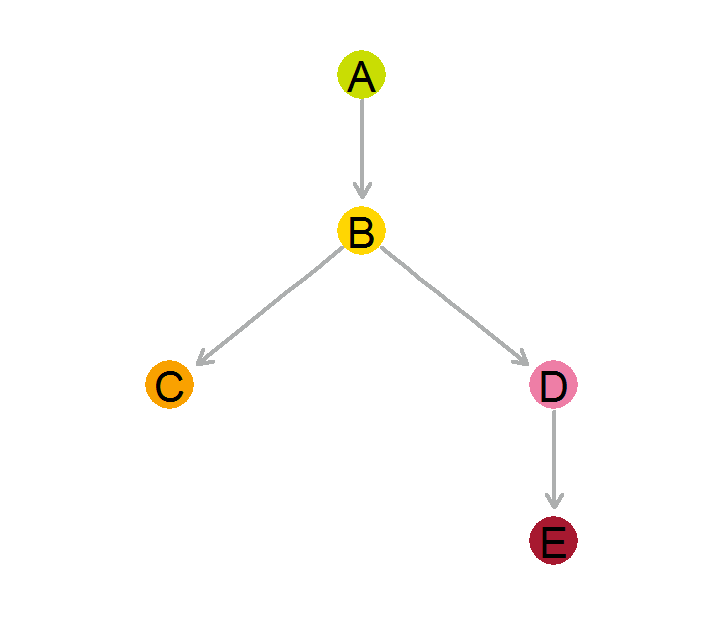
\includegraphics{gaga_hidden_data_phylogeny.png}
    \caption{The phylogeny of the optimum solution to the hidden data set.  Clone B is both the child of clone A and the parent of all other clones.}
\end{figure}

\begin{figure}[H]
   \centering
       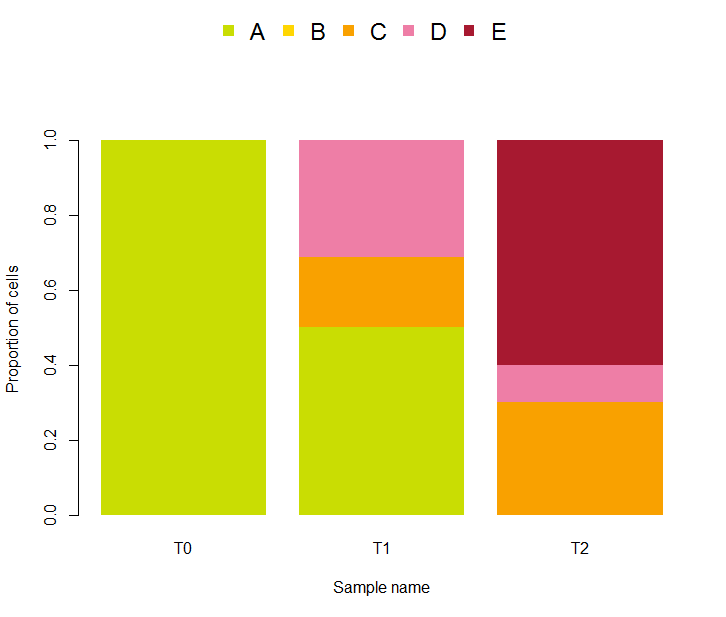
\includegraphics{gaga_hidden_data_proportions}
   \caption{The proportions of each clone in each sample of the hidden data set.  Although clone B is not present in any of the samples its existance and ancestry have been correctly inferred.}
\end{figure}

\subsection{Example 3 - complex synthetic data and noisy synthetic data}
These synthetic data are close to the sort of observations produced by a typical tumour-normal paired exome sequencing experiment.  There are four time points (T0 to T3) and 90 mutations (gene1 to gene90).  Each of the values represents the proportion of cells that contain that mutation at that time point - the cancer cell fraction (CCF).  {\color{red}We also include the same data set with added noise (HOW DID WE DO THIS - ASKED ALEX)}


\begin{Schunk}
\begin{Sinput}
> ## Load library
> library(GAGA)
> ## Load hidden data set
> data("gaga_synthetic_data")
> data("gaga_synthetic_data_jittered")
> ## Execute gaga() function on the synthetic data set
> hiddenDataSolution=gaga(gaga_hidden_data, number_of_clones=5, nroot=1,iterations=3000)
> ## Access solution slot in returned object to show highest scoring solution(s)
> ## This solution's score is -0.02500000
> hiddenDataSolution@solution
\end{Sinput}
\end{Schunk}
% Note; this R code snippet isn't in a regular knitr code block on purpose to make it appear as if it has been run
\begin{alltt}
     x1 x2 x3 x4 x5 x6 x7 x8 x9 x10 x11 x12 x13 x14 x15 x16 x17 x18 x19 x20 x21 x22 x23 x24 x25
[1,]  0  1  2  2  4 29  0  0  0   0   8   0   3   5   0   0   0   6   2  12   1   2   4   3   5
\end{alltt}

\begin{Schunk}
\begin{Sinput}
> ## Produce plots for the phylogeny, heatmap and proportions in turn
> gagaReport(gaga_hidden_data,hiddenDataSolution,outType="phylogeny")
> gagaReport(gaga_hidden_data,hiddenDataSolution,outType="heatmap")
> gagaReport(gaga_hidden_data,hiddenDataSolution,outType="proportion")
> ## Create output files representing the solution(s) in the current working directory
> gagaReport(gaga_simple_data,simpleDataSolution,outType="complete")
\end{Sinput}
\end{Schunk}



JITTERED DATA

\subsection{Example 4}
The yeast data, as it's REAL data and has a (relatively) definite answer AND is contaminated.
\subsection{Example 5}
Perhaps include the data from the recent LM paper?
\subsection{Advanced GAGA usage and best practices}
Demonstrate proper usage; how to iterate over many clones and estimate how many clones there are, then performing many runs
 and that the number of clones is probably the most important variable.  The user MUST cycle through a number of clones and choose the lowest number of clones with the best answer

\section{Session Info}
\begin{Schunk}
\begin{Sinput}
> sessionInfo()
\end{Sinput}
\begin{Soutput}
R version 3.0.2 (2013-09-25)
Platform: x86_64-w64-mingw32/x64 (64-bit)

locale:
[1] LC_COLLATE=English_United Kingdom.1252 
[2] LC_CTYPE=English_United Kingdom.1252   
[3] LC_MONETARY=English_United Kingdom.1252
[4] LC_NUMERIC=C                           
[5] LC_TIME=English_United Kingdom.1252    

attached base packages:
[1] stats     graphics  grDevices utils     datasets  methods   base     

other attached packages:
[1] GAGA_0.2

loaded via a namespace (and not attached):
[1] tools_3.0.2
\end{Soutput}
\end{Schunk}

\section{References}

\end{document}
